\documentclass[10pt,a4paper,twocolumn]{article}
\usepackage[margin=19mm,columnsep=7mm]{geometry}
\usepackage[T1]{fontenc}
\usepackage[utf8]{inputenc}
\usepackage{lmodern}
\usepackage{microtype}
\usepackage{amsmath,amssymb}
\usepackage{graphicx,booktabs,tabularx,longtable,array}
\usepackage{xcolor}
\usepackage{enumitem}
\usepackage{caption}
\usepackage{fancyhdr}
\usepackage{hyperref}
\definecolor{ink}{HTML}{132B45}
\definecolor{teal}{HTML}{176D80}
\hypersetup{colorlinks=true,linkcolor=ink,urlcolor=teal,citecolor=teal,
 pdftitle={Earth Detective: Regional Trends in NASA Earth Science Data},pdfauthor={Team Neural Newtons}}
\captionsetup{font=small,labelfont=bf}
\setlist{nosep,leftmargin=*}
\setlength{\parindent}{1em}
\setlength{\parskip}{2pt}
\setlength{\emergencystretch}{1.5em}
\pagestyle{fancy}
\fancyhf{}
\fancyhead[L]{\small\textsc{Earth Detective}}
\fancyhead[R]{\small Team Neural Newtons}
\fancyfoot[C]{\small\thepage}
\setlength{\headheight}{14pt}
\newcommand{\unitno}{\ensuremath{10^{15}\,\mathrm{molecules\,cm^{-2}}}}
\newcommand{\code}[1]{\texttt{#1}}
\newcommand{\TotalCacheValues}{35,748}
\newcommand{\TestCount}{38}
\newcommand{\SenError}{0}
\newcommand{\ParisTempSlope}{+0.396}
\newcommand{\ParisTempCI}{\ensuremath{[+0.260,\ +0.558]}}
\newcommand{\ParisRainSlope}{-0.036}
\newcommand{\ParisRainP}{0.707}
\newcommand{\LANoSlope}{-4.593}
\newcommand{\LANoCI}{\ensuremath{[-6.017,\ -3.808]}}
\newcommand{\DhakaNoSlope}{+1.593}
\newcommand{\DhakaNoCI}{\ensuremath{[+0.859,\ +2.237]}}
\newcommand{\SvalbardSlope}{+0.701}
\newcommand{\ArcticRatio}{1.77}
\newcommand{\BeijingEarlyP}{0.230}
\newcommand{\BeijingLaterSlope}{-7.735}
\newcommand{\BeijingLaterP}{\ensuremath{<0.001}}
\newcommand{\PairDifferences}{3}
\newcommand{\HRDifferences}{2}

\begin{document}
\twocolumn[{
\begin{center}
{\small\textsc{NASA Space Apps Challenge 2026}}\\[6pt]
{\LARGE\bfseries Earth Detective}\\[5pt]
{\Large A Transparent Tool for Regional Trends\\in NASA Earth Science Data}\\[10pt]
{\large Team name : Neural Newtons}\\[4pt]
{\small Kenza HASSANI \quad Eric CHEN \quad Elom OKOUMASSOUN \quad Ashneel BHAGOBAN}\\[5pt]
{\small Challenge: Be An Earth System Trend Detective!}\\[3pt]
{\Large\bfseries Technical project report}
\end{center}
\vspace{3pt}
\begin{minipage}{\textwidth}
\textbf{Abstract.}
Earth Detective helps users investigate changes in NASA Earth science data. A user selects a variable, a region and a time interval. The tool shows the monthly series, removes the average seasonal cycle and estimates the trend. It reports its direction, its rate per decade, a 95\% confidence interval and a Mann--Kendall p-value. We use four variables from three NASA products: air temperature and specific humidity from MERRA-2, precipitation from GPM IMERG, and tropospheric nitrogen dioxide from OMI on Aura. The data were extracted through NASA Giovanni and its area-averaging service through Harmony. The reviewed release contains 86 cached series, covering 43 variable--region combinations in 11 regions. Half are regional averages and half are grid-point series. The regional series support the main interface. All cached monthly calendars were checked. The application combines a Python statistical backend, a browser-based 3D globe, interactive charts and an optional language-model assistant. The assistant receives computed results rather than producing the statistical verdict. Worked examples show opposite NO$_2$ trends in Los Angeles and Dhaka, and a stronger temperature increase in Svalbard than in Paris. The project aims to make environmental evidence easier to explore, explain and check. The application is publicly available at \url{https://earth-detective.onrender.com} and its source code at \url{https://github.com/elomokm/Neural_newtons_nasa_sp}.\\[5pt]
\textbf{Keywords:} Earth science, NASA Giovanni, MERRA-2, IMERG, OMI, trend analysis, Mann--Kendall, Sen's slope, scientific communication.
\end{minipage}
\vspace{13pt}
}]

\section{Introduction}
\subsection{The problem}
Earth science datasets contain many variables, several spatial scales and different time resolutions. A line chart can show change, but it does not tell a user whether a visible pattern is a seasonal cycle, a short fluctuation or a persistent trend. The same variable can also increase in one region and decrease in another.

The Space Apps challenge asks for a tool that lets users select Earth science variables, obtain data for a region, display a time series and estimate the size and statistical significance of change \cite{challenge}. We designed Earth Detective around these four tasks.

Our intended users are high-school students, university students and members of the public with an interest in environmental data. They should be able to ask a question, inspect the observations and understand why the tool reaches a particular result.

\subsection{Our approach}
We built a guided investigation rather than a collection of disconnected plots. Each result follows the same chain: a named NASA product, a defined region, a selected period, a statistical calculation and a short explanation. The user can inspect the detailed tests and export the data.

The physics enters through the NASA products, the meaning of each variable and the unit conversions. Statistical methods estimate the trends. An optional AI layer helps users choose an investigation and understand its output. These roles remain separate. A language model does not supply the slope, confidence interval or p-value.

The current release focuses on 11 selected regions. The globe provides geographic context and navigation. It does not represent complete statistical coverage of every country. The regions were chosen to include urban, agricultural, tropical, semi-arid, Mediterranean and Arctic settings.

\subsection{What we built}
The implemented system provides:
\begin{enumerate}
\item Four variables with source identifiers, units and short definitions.
\item Monthly observations and season-adjusted views for cached regions.
\item Trend direction, Sen's slope, a confidence interval and significance testing.
\item A globe atlas and side-by-side regional comparisons.
\item Four guided investigations, data exports and shareable view settings.
\item Trendbot, with an optional language model and a rule-based fallback.
\end{enumerate}
The following sections describe the reviewed implementation and its measured outputs. Planned extensions are identified separately.

\section{User workflow}
A user first chooses a variable, such as precipitation, or asks a question in Trendbot. The application suggests a supported variable and region. The user can also search for a region or select one on the globe.

The date controls restrict the analysis to the available record. The backend then reads the cached series, calculates the anomalies and annual values, and runs the trend analysis. The interface displays a rise, a fall or an inconclusive result at the chosen significance threshold.

The time-series chart has two views: monthly values and monthly anomalies. The user can show the fitted trend line. A second region can be added for comparison with the same variable. A details view exposes the source, period, sample size, tests and export options.

The guided cases cover three outcomes in Paris, opposite NO$_2$ trends in Los Angeles and Dhaka, a change of study period in Beijing, and a temperature comparison between Svalbard and Paris. The case definitions select inputs. Their numerical conclusions come from the backend.

\section{NASA data and resources}
\subsection{NASA resources used in the project}
NASA data are the input to the analysis, not only the background of the interface. We use three NASA Earth science products obtained through Giovanni, a service operated by NASA Goddard Earth Sciences Data and Information Services Center, or GES DISC \cite{giovanni}. Harmony handles the regional area-averaging requests \cite{harmony}.

The four exact Giovanni identifiers and dataset DOIs are listed in Appendix~\ref{app:products}. We checked the product titles, versions and DOIs against NASA's Common Metadata Repository during the preparation of this report. The cache manifest links each processed series to its variable, region, source unit and extraction run.

NASA Blue Marble imagery is also used on the globe. It is a visual resource. The texture is not used to calculate temperature, precipitation, humidity or pollution trends. The statistical inputs come from the numerical products described below.

\subsection{Air temperature and specific humidity}
We use MERRA-2 collection \code{M2IMNXASM}, version 5.12.4, for \code{T2M} and \code{QV2M}. MERRA-2 is a NASA atmospheric reanalysis. It combines observations with a numerical model \cite{merra,gelaro}.

\code{T2M} is air temperature at 2~m. It is stored in kelvin and displayed in degrees Celsius. It is different from satellite land-surface temperature. \code{QV2M} is specific humidity at 2~m. It is stored in kg/kg and displayed in g/kg. It describes water-vapour mass per unit mass of moist air. It is not relative humidity.

Both records cover January 1980 to December 2024 in our cache, giving 540 monthly values per region. The native grid is 0.5 degrees in latitude by 0.625 degrees in longitude. A city label therefore refers to a model region or grid cell, not a street-level measurement.

The selected collection contains monthly means of instantaneous diagnostics. We retain its exact identifier rather than treating it as interchangeable with other MERRA-2 monthly collections.

\subsection{Precipitation}
We use GPM IMERG Final Run monthly precipitation, collection \code{GPM\_3IMERGM}, version 07 \cite{imerg}. IMERG combines information from several satellites to estimate precipitation. Our cached record covers January 1998 to December 2024, or 324 months per region.

The source unit is mm/hour. We multiply by 24 to display the monthly mean precipitation rate in mm/day. This quantity is a rate, not a monthly or annual accumulated rainfall total. Its trend unit is therefore mm/day per decade.

IMERG has a 0.1-degree grid. This differs from the MERRA-2 grid. The application compares their separate trends without claiming that the products share the same spatial resolution or error structure. The exact version and period are part of the result provenance.

\subsection{Tropospheric nitrogen dioxide}
We use the OMI/Aura \code{OMNO2d} daily level-3 product, version 003, and its cloud-screened tropospheric column variable \cite{omi}. OMI measures a column amount above an area. It does not directly measure the NO$_2$ concentration breathed at ground level.

The source unit is molecules/cm$^2$. We scale it by $10^{-15}$ for display in \unitno. Daily values are averaged into monthly values. At least five valid daily values are required for a monthly mean.

The monthly cache runs from October 2004 to December 2024. The main annual analysis begins in 2005 because the three months of 2004 do not meet the annual inclusion rule. The product grid is 0.25 degrees. OMI is not included for Svalbard in our release. Polar darkness and limited retrieval availability make this an unsuitable demonstration combination.

\subsection{Regions and cache coverage}
The catalogue contains Paris, the Po Valley, Beijing, Los Angeles, Dhaka, Delhi, the Sahel, Svalbard, central Spain, central Amazonia and a rectangle around metropolitan France. Appendix~\ref{app:regions} gives the extraction bounds.

Each combination normally has a regional average and a grid-point record. The exception is NO$_2$ at Svalbard. The resulting cache contains 43 regional series and 43 point series. The default loader prefers the regional series when both exist.

A regional series is the area-average service output for a bounding box. It is not an average clipped to a national boundary. This distinction is important for the region labelled France and for boxes that include water or neighbouring territories. We do not infer a complete national monitoring system from these data.

\begin{table*}[t]
\centering\small
\caption{Data included in the reviewed cache. The numbers are based on an audit of the actual CSV files. The two origins are regional average and grid point.}
\label{tab:data}
\begin{tabularx}{\textwidth}{@{}l l l r r X@{}}
\toprule
Variable & NASA product & Cached period & Months & Regions & Display unit \\
\midrule
Air temperature & MERRA-2 & 1980-01 to 2024-12 & 540 & 11 & $^\circ$C \\
Specific humidity & MERRA-2 & 1980-01 to 2024-12 & 540 & 11 & g/kg \\
Precipitation rate & GPM IMERG V07 & 1998-01 to 2024-12 & 324 & 11 & mm/day \\
Tropospheric NO$_2$ & OMI/Aura V003 & 2004-10 to 2024-12 & 243 & 10 & \unitno \\
\bottomrule
\end{tabularx}
\end{table*}

\section{Data processing}
\subsection{Acquisition}
The ingestion code offers two paths. The point path calls the Giovanni Time Series API and reads the nearest grid point. The regional path resolves the collection in CMR, submits an asynchronous Harmony request and downloads the area-average CSV. The request contains the collection, variable, time bounds and bounding box.

Data acquisition runs separately from visitors' sessions. The hosted application reads prepared NASA series, so users can explore the results directly in the browser without configuring the data pipeline.

The ingestion script can select variables, regions and origin type. It can run several extraction jobs in parallel. Raw responses are saved separately when rebuilding the cache. This makes it possible to check parsing and conversions without requesting the data again.

\subsection{Parsing and missing values}
The point parser finds the timestamp header instead of assuming a fixed number of metadata lines. The regional parser separates the metadata block from the data table. Declared fill values are masked as missing values. The parser also masks extremely large sentinel-like magnitudes.

The area-average response may not contain a unit. The code first queries CMR variable metadata. If that metadata is unavailable, it reads the unit from a short point request for the same product. This fallback is used for the precipitation product.

Monthly timestamps are set to the first day of each month. The expected monthly index is rebuilt between the catalogue start and December 2024. Months that have no value remain missing. The runtime normalizer keeps the first occurrence of a repeated monthly index. Our separate cache audit checks for duplicates before accepting the packaged data.

\subsection{Unit conversions}
The transformations are explicit:
\begin{align}
T_{\mathrm{C}} &= T_{\mathrm{K}}-273.15,\\
q_{\mathrm{g/kg}} &= 1000q_{\mathrm{kg/kg}},\\
P_{\mathrm{mm/day}} &= 24P_{\mathrm{mm/hour}},\\
N_{15} &= 10^{-15}N_{\mathrm{molecules/cm^2}}.
\end{align}
The converter checks the expected source-unit family. An unexpected unit raises an error. This prevents a rate, a temperature or a column amount from being silently interpreted in the wrong unit.

\subsection{Monthly NO$_2$ and data storage}
For a month $m$, the NO$_2$ processing rule is
\begin{equation}
\bar x_m=\frac{1}{d_m}\sum_{d\in D_m}x_d,
\qquad d_m=|D_m|\geq5.
\end{equation}
Here $D_m$ contains the valid daily values. If fewer than five days are available, the monthly value is missing. This is a minimum data-availability rule. It does not guarantee uniform daily sampling or eliminate cloud-related sampling effects.

Each processed CSV contains a date, a converted value and a display unit. The manifest records valid and missing counts, source identifiers and acquisition details. The application reads this prepared data cache. Its main scientific workflow therefore does not depend on a live NASA request during a demonstration.

\section{Statistical methods}
\subsection{Period selection and seasonal adjustment}
Let $x_{y,m}$ be the monthly value for year $y$ and calendar month $m$. The backend first selects the user's period. It then calculates the mean of each calendar month over that selected period:
\begin{equation}
\mu_m=\frac{1}{n_m}\sum_{y\in Y_m}x_{y,m},
\qquad a_{y,m}=x_{y,m}-\mu_m.
\label{eq:anomaly}
\end{equation}
The anomaly $a_{y,m}$ describes the difference from the average January, February and so on. The reference is recalculated when the study period changes. It is not a fixed external climate-normal period.

This adjustment removes the mean annual cycle. It does not remove every form of seasonality or dependence. It also does not make observations independent.

\subsection{Annual analysis series}
The test uses the mean monthly anomaly in each eligible calendar year:
\begin{equation}
A_y=\frac{1}{k_y}\sum_{m\in M_y}a_{y,m},
\qquad k_y=|M_y|\geq10.
\label{eq:annual}
\end{equation}
The implementation uses equal weights for valid months and accepts years with at least ten months. It does not use day-weighted annual means. This is the method used by the final application, which differs from the stricter 12-month rule in the earlier exploratory notebook.

Annual aggregation reduces the direct effect of neighbouring monthly observations on the primary test. It does not guarantee that neighbouring years are independent. The backend requires a span of at least five years and at least five eligible annual values. The interface also flags records shorter than 30 years.

\subsection{Mann--Kendall test}
For $n$ annual anomalies ordered by year, the Mann--Kendall statistic is
\begin{equation}
S=\sum_{i=1}^{n-1}\sum_{j=i+1}^{n}\operatorname{sgn}(A_j-A_i).
\end{equation}
Positive and negative pairwise differences contribute $+1$ and $-1$. Equal values contribute zero. The tie-corrected variance is
\begin{equation}
V_S=\frac{n(n-1)(2n+5)-\sum_g t_g(t_g-1)(2t_g+5)}{18},
\end{equation}
where $t_g$ is the size of tie group $g$. The continuity-corrected normal statistic is
\begin{equation}
Z=\begin{cases}
(S-1)/\sqrt{V_S}, & S>0,\\
0, & S=0,\\
(S+1)/\sqrt{V_S}, & S<0.
\end{cases}
\end{equation}
The two-sided p-value is
\begin{equation}
p=2\left[1-\Phi(|Z|)\right].
\end{equation}
The application uses $\alpha=0.05$. It reports a significant trend when $p<\alpha$. The calculations use \code{pymannkendall} \cite{mann,pymk}.

A p-value is evaluated under the test's null hypothesis and assumptions. It is not the probability that the trend is false. A result above 0.05 means that this test did not detect a trend at that threshold. It does not establish stability.

\subsection{Sen's slope}
Mann--Kendall tests ordering. Sen's estimator gives the rate of change \cite{sen}. With the actual calendar years $t_i$, we calculate
\begin{equation}
b_{ij}=\frac{A_j-A_i}{t_j-t_i},
\qquad \hat\beta=\operatorname{median}_{i<j}(b_{ij}).
\end{equation}
Using the year differences preserves the time interval if an annual value is excluded. The displayed rate is
\begin{equation}
\hat\beta_{10}=10\hat\beta.
\end{equation}
The unit stays attached to the variable. For example, a temperature rate is in $^\circ$C per decade. A precipitation-rate trend is in mm/day per decade. Median-based estimation reduces sensitivity to individual extreme observations, but it is not immune to data errors or structural changes.

\subsection{Confidence interval and trend line}
The code forms a 95\% slope interval from the sorted pairwise slopes and the Mann--Kendall variance \cite{gilbert,usgs}. If $N=n(n-1)/2$ and $C=1.959964\sqrt{V_S}$, its interpolated rank bounds are
\begin{equation}
r_L=(N-C)/2,\qquad r_U=(N+C)/2+1.
\end{equation}
Ranks are clipped to the range 1 to $N$. The corresponding slope values are multiplied by ten for display. This interval uses the original test variance. It is not automatically adjusted when a secondary autocorrelation test gives a different result.

For plotting, the intercept is the median annual residual:
\begin{equation}
\hat\alpha=\operatorname{median}_i(A_i-\hat\beta t_i),
\qquad \hat A(t)=\hat\alpha+\hat\beta t.
\end{equation}
The slope-based total change is $\hat\beta$ times the selected duration. It is a fitted change over the period, not simply the last observed month minus the first.

\subsection{Secondary checks and period sensitivity}
The details output also includes a Hamed--Rao modified Mann--Kendall test on annual values, a seasonal Mann--Kendall test on monthly anomalies, and an ordinary least-squares comparison \cite{hamed,hirsch,pymk}. These are diagnostic checks. They do not replace the primary verdict automatically.

The seasonal implementation groups observations in blocks of 12 and trims any trailing incomplete block. Its interpretation therefore needs care when the selected record begins partway through a calendar year. Full January-to-December periods are the clearest comparison setting.

The backend also exposes a start-year sensitivity endpoint. It repeats the same analysis with later start years and a common end date. This shows that a trend is a statement about a specified interval. It is not an automatic change-point detector, and trying many intervals can affect false-positive risk.

\section{Software architecture}
\subsection{Separation of responsibilities}
The system has three main layers. The data layer reads a small catalogue and a prepared data cache. The scientific layer returns one shared result structure. The browser layer renders that result and handles user interaction.

The result object contains the source series, selected bounds, anomalies, trend line, slope per decade, confidence interval, p-value, direction, total fitted change, short-period flag, summary and test table. Both the web API and the fallback Streamlit application use the same backend entry point.

The browser formats values for display and export. It does not recalculate the primary significance test. This keeps the numerical result consistent between charts, cards, comparisons and the assistant context.

\begin{figure*}[t]
\centering
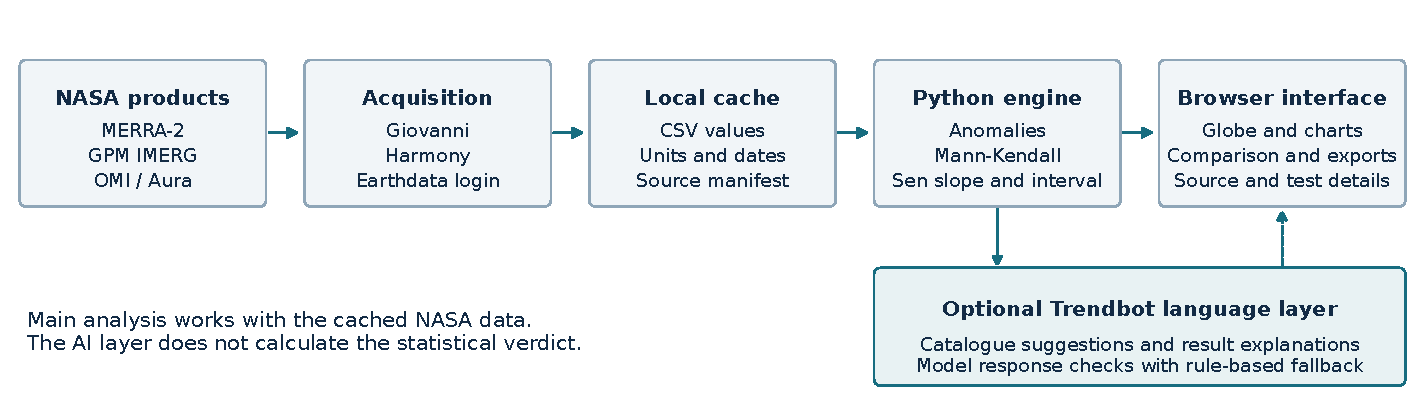
\includegraphics[width=\textwidth]{figures/architecture.pdf}
\caption{Implemented data and computation flow. The optional AI path receives the catalogue or an already computed result. Cached NASA data remain sufficient for the main statistical workflow.}
\label{fig:architecture}
\end{figure*}

\subsection{Python backend and API}
Python handles CSV reading, calendar alignment, unit conversion and statistics. Pandas manages the time series. NumPy supports numerical operations. SciPy provides the least-squares diagnostic. \code{pymannkendall} provides the test family.

FastAPI exposes the catalogue, analysis and assistant routes as JSON. Uvicorn serves the API and the built frontend. Non-finite values are converted to JSON \code{null}. Unknown identifiers, missing cached series and invalid study periods produce explicit HTTP errors.

The backend caches series and results in memory using least-recently-used caches. A result key includes the variable, region and selected dates. Repeated views can therefore reuse a calculation. This is a responsiveness measure, not a claim about a measured deployment throughput.

\subsection{Browser interface}
The frontend uses JavaScript, HTML and CSS. Three.js renders the WebGL globe. D3 draws the charts. World Atlas and TopoJSON provide geographic boundaries and labels for navigation. Esbuild creates the distribution bundle.

The interface is available in French and English, including region names, variable definitions, guided investigations, the plain-language verdict and the test table. Monthly and annual CSV exports preserve the selected data view. The URL hash stores the main view settings for sharing. Local storage keeps interface preferences.

A globe click selects a nearby catalogue region when one is available. It does not request arbitrary national statistics. The backend contains a live point-retrieval function, but this is not the default public analysis path in the reviewed frontend.

\subsection{Public access and deployment}
Earth Detective is deployed as a public website at \url{https://earth-detective.onrender.com}. Visitors choose a variable, a supported region and a period on the site. The hosted FastAPI backend reads the prepared NASA series and returns the analysis to the browser. Visitors do not need to install the development tools or manage the data acquisition pipeline. The service runs on a free Render instance described by a versioned configuration file in the repository, and it is redeployed automatically from the main branch. On the free tier the instance sleeps after a period of inactivity, so the first request after a pause can take about a minute. The source code is available at \url{https://github.com/elomokm/Neural_newtons_nasa_sp}. The verification in this report assesses the application and its data, rather than the availability or capacity of the hosting service.

\subsection{Development tools and hardware}
We developed the project with VS Code, Git, Python and Node.js. The Python dependencies are declared in the project files. The frontend dependencies are declared in its package file. Appendix~\ref{app:software} records the versions used for this verification.

The core analysis runs on a standard computer with a CPU. The globe needs a browser with WebGL support. No custom sensor, special acquisition hardware or trained GPU model is part of the system. The NASA products supply the environmental observations and model-based estimates. We do not claim specific hardware performance without a controlled benchmark.

\section{Trendbot and the AI layer}
\subsection{Two supported operating modes}
Trendbot helps with two tasks: choosing a supported investigation and explaining the result currently shown. The optional model connection uses the OpenAI Python SDK. Its default model setting is \code{gpt-4.1-mini}, and the model can be changed by configuration.

When the optional model service is unavailable or a request fails, rules recognise variable keywords and region aliases. Explanations are assembled from the statistical result. The cached analysis remains usable without paid model access.

No model is trained on the NASA cache in this release. The AI component is a language interface around a statistical tool. The numerical model and scientific result do not depend on text generated by the assistant.

\subsection{Context and output checks}
The model receives a restricted catalogue for suggestions. The returned identifiers are checked against the catalogue and against the variables available in a region. A result explanation receives the actual slope, confidence bounds, p-value, period and unit.

The application checks numerical tokens against allowed result values and applies vocabulary checks to unsupported claims of proof or stability. Invalid responses are rejected and the fallback is used. Model timeouts and exceptions also trigger fallback behaviour.

These checks reduce some failure modes. They are not a formal guarantee of factual correctness. In particular, the current numeric check compares magnitudes and tolerates rounding. It does not independently prove that every sign, unit or causal phrase is correct. The result cards remain tied to the backend's numeric fields. We did not run live paid-model calls as part of the report verification.

\section{Verification and results}
\subsection{Evaluation scope}
We reviewed the source code, product catalogue, region definitions, cache manifest, statistical engine, API adapter, frontend and assistant integration. We then ran the repository tests and recalculated every available regional analysis from the cached CSV files.

The evaluation uses a versioned snapshot of the release pulled on 15 November 2026. File hashes are saved with the accompanying evidence. We did not redownload all NASA products during this review. The tests verify the packaged data and the software behaviour. They do not constitute an independent validation of the satellite retrievals or the reanalysis.

\subsection{Cache audit and software tests}
The cache contains \TotalCacheValues{} monthly rows across 86 CSV files. The audit checked the expected calendar for each product, duplicate dates, missing values, non-finite values and unit labels. All 86 series have the expected monthly calendar and no duplicate dates. All 43 regional-average series have valid values in every expected month. Five NO$_2$ point series contain 31 missing monthly values in total. These are retained as missing values. Calendar completeness and value completeness are therefore reported separately. These checks apply only to the listed regions and product periods. They do not mean that every underlying daily retrieval was present.

The repository test run completed with \TestCount{} passing tests. Tests cover unit conversions, monthly aggregation, cache precedence, missing-month representation, catalogue behaviour, synthetic trend recovery, assistant fallback and the API. Synthetic fixtures test controlled cases. They are not mixed into the NASA result tables.

As an additional numerical check, we compared all 43 annual Sen slope estimates with SciPy's independent Theil--Sen implementation. The maximum absolute difference was \SenError{} in display units per decade. This verifies the slope calculation on these inputs. It is not a separate validation of the confidence-interval calibration.

\subsection{Paris: three different outcomes}
On the full cached periods, Paris has a temperature trend of \ParisTempSlope{} $^\circ$C per decade, with a 95\% interval of \ParisTempCI{}. The test detects an increase at the 5\% threshold. Specific humidity also increases.

The Paris NO$_2$ series shows a decrease. The precipitation-rate estimate is \ParisRainSlope{} mm/day per decade, with p-value \ParisRainP{}. This test does not detect a precipitation trend at the chosen threshold. The tool therefore supports different answers in the same place, depending on the variable.

\subsection{The same variable, opposite regional directions}
For NO$_2$, Los Angeles has a Sen slope of \LANoSlope{} \unitno{} per decade, with a 95\% interval of \LANoCI{}. Dhaka has a slope of \DhakaNoSlope{} in the same unit, with an interval of \DhakaNoCI{}. Both are significant in the primary test. Their directions are opposite.

This is a direct demonstration of the challenge's regional question. It does not establish that the two changes have the same cause. It also does not translate the column trends into a quantified health impact.

\begin{figure*}[t]
\centering
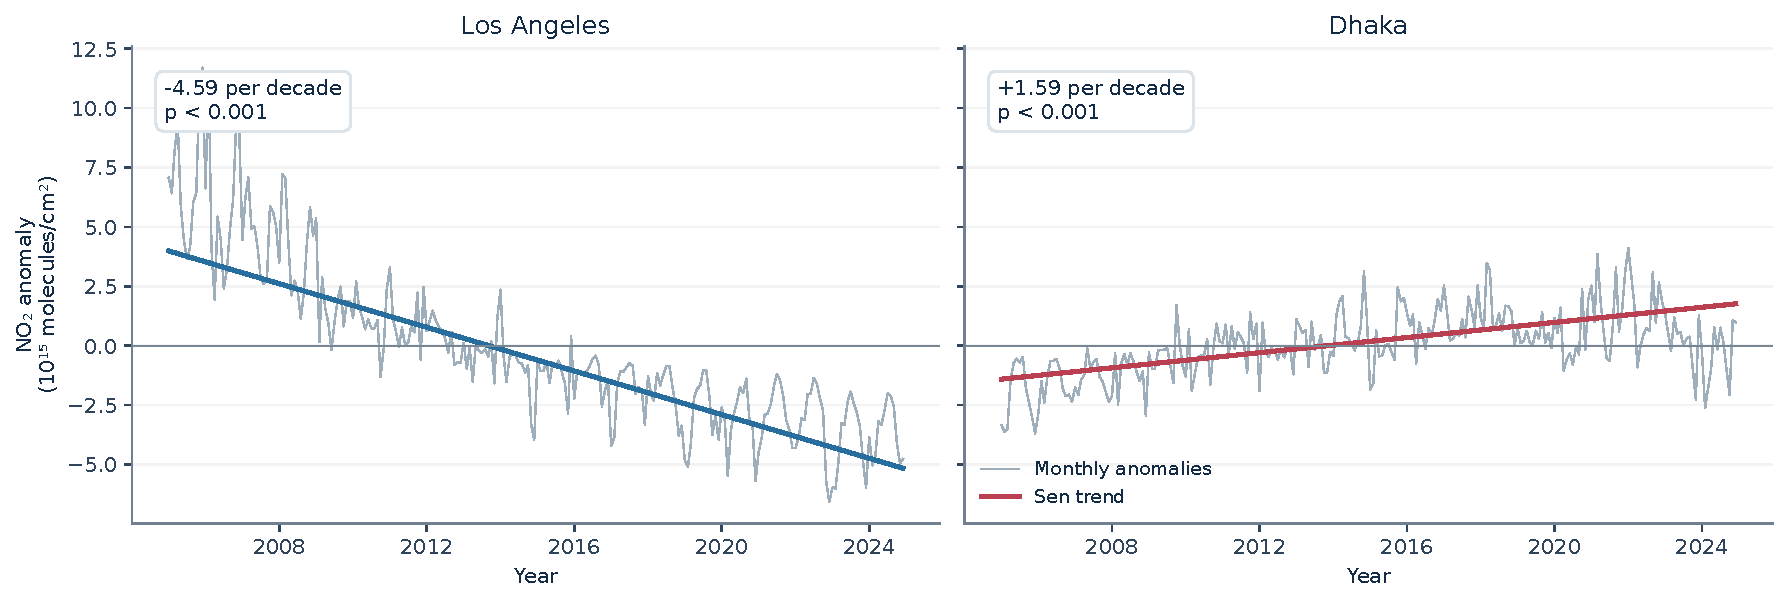
\includegraphics[width=\textwidth]{figures/no2_comparison.pdf}
\caption{Recomputed OMI NO$_2$ anomalies and Sen trend lines, displayed from 2005 to 2024. Each region uses its own monthly reference means from the full cached record, which starts in October 2004. Only 2005 to 2024 meet the annual inclusion rule. The two panels share the same unit. The trends are estimated from annual mean anomalies, while the light curves show monthly anomalies.}
\label{fig:no2}
\end{figure*}

\subsection{Svalbard and Paris}
For 1980 to 2024, the temperature slope is \SvalbardSlope{} $^\circ$C per decade in Svalbard and \ParisTempSlope{} $^\circ$C per decade in Paris. The ratio of the two point estimates is \ArcticRatio{}. Both primary tests detect an increase.

The ratio is a descriptive comparison of these two regional estimates. We have not performed a formal test of the difference between the slopes. It should not be presented as a new estimate for the whole Arctic.

\subsection{Beijing and the selected interval}
The guided NO$_2$ case compares 2005 to 2011 with 2012 to 2024. The earlier interval gives p = \BeijingEarlyP{}. The later interval gives a slope of \BeijingLaterSlope{} \unitno{} per decade and p \BeijingLaterP{}.

The example shows sensitivity to the selected interval. It does not identify a change point automatically or attribute the later decline to a policy. The intervals are demonstration choices, so their tests should not be interpreted as a prospectively registered causal study.

\subsection{Region averages and grid points}
The two origins produce different primary verdicts in \PairDifferences{} of the 43 matched combinations. These cases are listed in the evidence table. This shows why spatial support must remain visible. A point estimate and a regional average answer different questions.

The main application uses the regional average when it is available. It does not combine the point and area-average values into a single measurement or treat agreement as proof of accuracy.

\subsection{Diagnostic agreement}
The Hamed--Rao diagnostic and the primary test disagree at the 5\% threshold for \HRDifferences{} of the 43 regional combinations. The diagnostic values are available in the result output. The primary test still controls the displayed verdict in this release.

Disagreement is useful information. Annual aggregation reduces monthly dependence, but it does not remove all serial correlation. We report the implemented decision rule and its checks rather than claiming that every significant result is robust to every statistical choice.

\begin{figure*}[t]
\centering
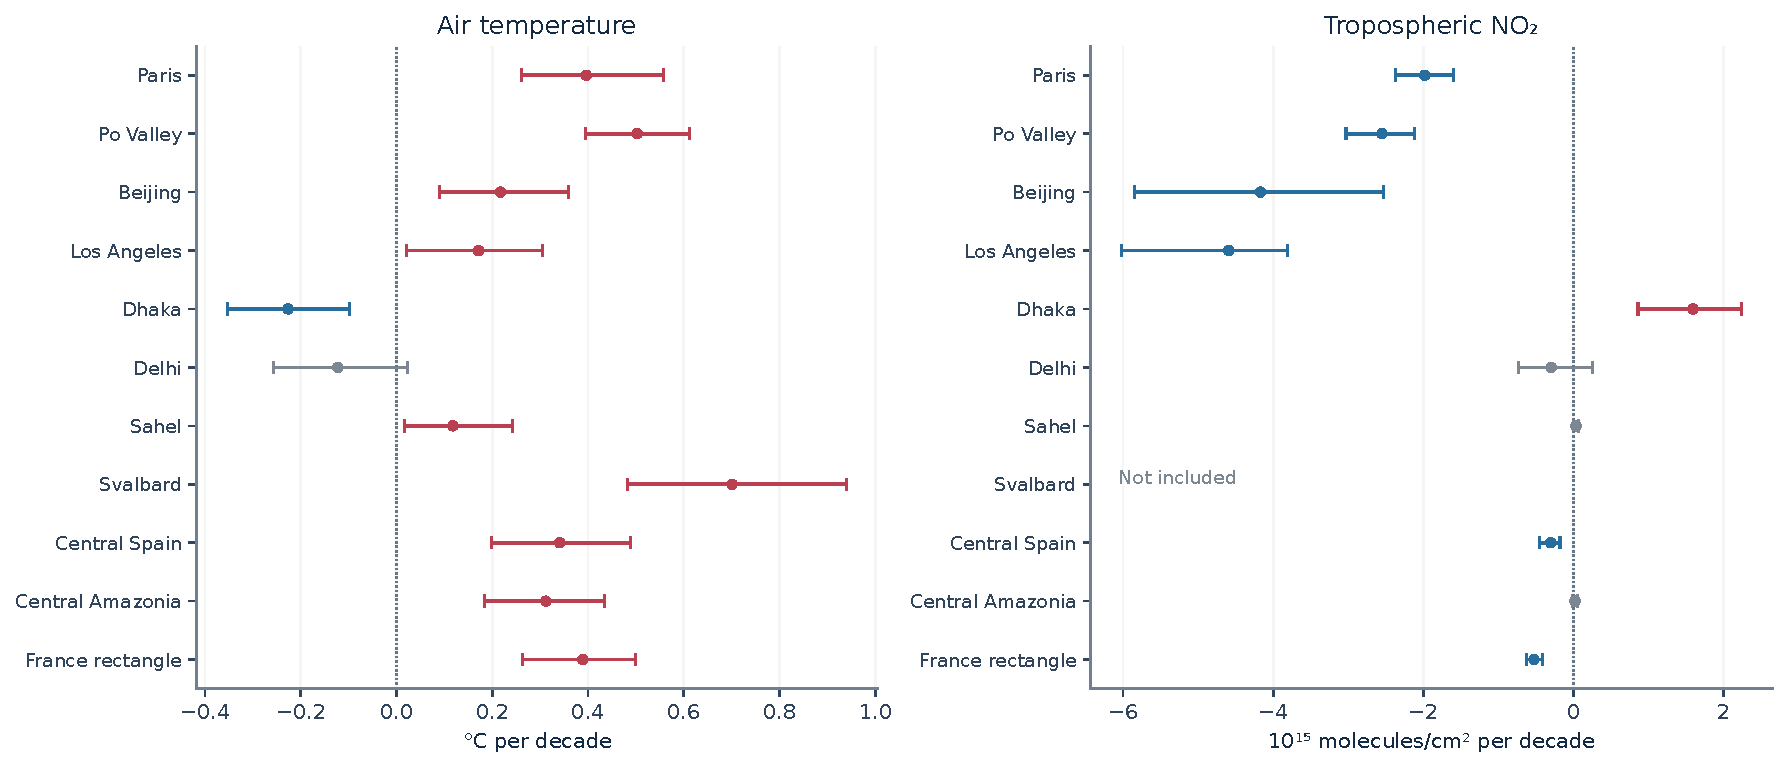
\includegraphics[width=\textwidth]{figures/regional_slopes.pdf}
\caption{Regional temperature and NO$_2$ slopes with the confidence intervals returned by the engine. Grey markers indicate a primary p-value of at least 0.05. Red and blue identify significant rises and falls. Svalbard has no NO$_2$ series in the catalogue. The 43 full results are listed in Appendix~\ref{app:results}.}
\label{fig:slopes}
\end{figure*}

\section{Design choices and originality}
The creative contribution is the investigation workflow. The globe, comparisons, guided cases, source details and assistant all lead back to the same computed result. A user can move from a broad question to the underlying observations without changing tools. Opposite regional trends become visible on the same screen.

We considered several constraints. A short hackathon favoured a small, tested catalogue over unsupported geographic coverage. NASA request time and authentication requirements led us to separate acquisition from interactive analysis. The audience led us to pair simple verdicts with technical details. Different product units and periods required explicit conversion and provenance. Dependence in time series led to annual testing and secondary checks. Optional model access required a fallback that works when the model service is unavailable.

These choices also shaped the interface. The globe provides context, while the chart carries the evidence. Rise, fall and inconclusive results have consistent visual meanings. The assistant helps with navigation and explanation, while the backend owns the calculations. We use established statistical methods and make their assumptions visible.

\section{Benefits and intended use}
\subsection{Making evidence accessible}
Earth Detective connects a simple question to a traceable scientific result. Users do not need to know a NASA product identifier before starting. They can begin with a place or question, then inspect the variable, source and method when they need more detail.

The anomaly view helps separate the average seasonal cycle from longer changes. Units and slopes give the result a physical scale. Confidence bounds show estimation uncertainty. The inconclusive outcome also has a clear place in the workflow. Users are not pushed towards a significant result.

\subsection{A reproducible teaching tool}
The packaged cache makes classroom and hackathon demonstrations less dependent on network access. Exports allow a student to inspect the values outside the application. Guided cases show how the same workflow applies to different products and regions.

The shared backend makes the calculations easier to maintain. A change to the statistical engine can be tested once and then reflected in the web interface and fallback application. The assistant can be replaced without changing the statistical result structure.

These benefits follow from the implemented design. We have not yet measured learning outcomes, user comprehension or adoption in a formal study. Those are goals for the next stage.

\section{Limitations}
\subsection{Data and spatial interpretation}
The release covers a selected catalogue, not every country. Bounding boxes may mix land, sea and neighbouring areas. The app does not recompute exact country-boundary averages or document monthly cell-level spatial coverage. Different NASA grids also limit direct local comparisons.

MERRA-2 estimates, IMERG precipitation and OMI column retrievals have different observation and modelling processes. Their uncertainty is not fully represented by a trend confidence interval. A complete processed monthly record does not demonstrate complete daily sampling or an unchanged spatial mask.

The five-day NO$_2$ rule and the ten-month annual rule are pragmatic minimums. Uneven sampling can still influence an average. For the current complete monthly cache, all full years meet the monthly rule, but OMI's partial first year is excluded.

\subsection{Statistical interpretation}
The primary Mann--Kendall test assumes an appropriate dependence structure under the null. The displayed interval uses its unmodified variance. Secondary tests expose sensitivity, but do not change the verdict. The application also does not apply a multiple-testing correction across the regional catalogue or across repeated period selections.

The estimated slope summarises a period. It is not a forecast, a physical attribution model or an automatic estimate of nonlinear change. A short record can support an exploratory trend analysis, but does not have the same temporal context as a longer climate record. The 30-year flag is a communication rule, not a universal validity test \cite{wmo}.

\subsection{Interface and AI}
The globe's geographic coverage is broader than the statistical catalogue. Selecting a named region or a nearby marker should not be confused with measuring any clicked location.

The optional AI checks are limited and require further evaluation. A model explanation can be fluent while missing context. The deterministic numeric output, source display and fallback path remain important. We do not report a hallucination rate or claim a fully validated AI safety system.

\section{Next steps}
Our first goal is to make the regional evidence easier to inspect. We plan to expose daily and spatial coverage information, improve warnings for partial-year selections, and present agreement between the primary and corrected tests more directly.

For wider coverage, we would add versioned national polygons and stable cell-intersection weights. Small islands, coastal regions and polar areas need explicit policies. We would extend the cache only after checking the variable definition, period and product support.

A second goal is statistical evaluation. We would test interval coverage on controlled autocorrelated series, assess sensitivity to missing months and compare multiple-testing strategies. Any forecasting or multivariable model would need a separate question and time-based validation.

For the assistant, we would evaluate sign, unit, scope and significance consistency on a fixed question set. User testing would then check whether the tool improves understanding of trends, uncertainty and non-significant results.

\section{Conclusion}
Earth Detective turns NASA Earth science records into regional investigations. It combines a defined data source, clear units, a selected time period, established trend methods and an interface that exposes the evidence. The current release uses actual MERRA-2, IMERG and OMI data extracted through Giovanni and Harmony.

The verified examples show that trend direction depends on both variable and region. They also show why period choice, spatial support and uncertainty must remain visible. Our aim is to help users ask better questions of NASA data and understand the limits of the answer.

\section*{Team and development statement}
Team Neural Newtons consists of Kenza HASSANI, Eric CHEN, Elom OKOUMASSOUN and Ashneel BHAGOBAN. The project brings software, physical interpretation and visual communication together. The optional assistant uses an existing language model. We do not claim to have trained a new foundation model. The team also used AI coding assistants, including Claude Code, to help write and review parts of the code, the documentation and this report. All code was reviewed and tested by the team, and every number in this report was recomputed from the cached data. No images, video or audio were generated with AI. This report describes a hackathon prototype and its software verification, not a peer-reviewed validation study.

\begin{thebibliography}{20}
\small
\bibitem{challenge} NASA Space Apps. \emph{Be An Earth System Trend Detective!} 2026. \url{https://www.spaceappschallenge.org/2026/challenges/earth-system-trend-detective/}.
\bibitem{giovanni} NASA GES DISC. \emph{Giovanni}. \url{https://giovanni.earthdata.nasa.gov/}. Accessed 15 November 2026.
\bibitem{harmony} NASA Earthdata. \emph{Harmony API documentation}. \url{https://harmony.earthdata.nasa.gov/docs}.
\bibitem{merra} Global Modeling and Assimilation Office. \emph{MERRA-2 instM\_2d\_asm\_Nx, version 5.12.4}. NASA GES DISC. \href{https://doi.org/10.5067/5ESKGQTZG7FO}{doi:10.5067/5ESKGQTZG7FO}.
\bibitem{gelaro} Gelaro, R., et al. The Modern-Era Retrospective Analysis for Research and Applications, Version 2. \emph{Journal of Climate}, 30, 5419--5454, 2017. \href{https://doi.org/10.1175/JCLI-D-16-0758.1}{doi:10.1175/JCLI-D-16-0758.1}.
\bibitem{imerg} Huffman, G. J., et al. \emph{GPM IMERG Final Precipitation L3 1 month 0.1 degree V07}. NASA GES DISC. \href{https://doi.org/10.5067/GPM/IMERG/3B-MONTH/07}{doi:10.5067/GPM/IMERG/3B-MONTH/07}.
\bibitem{omi} NASA GES DISC. \emph{OMI/Aura NO2 Cloud-Screened Total and Tropospheric Column L3 Global Gridded 0.25 degree V3}. \href{https://doi.org/10.5067/Aura/OMI/DATA3007}{doi:10.5067/Aura/OMI/DATA3007}.
\bibitem{mann} Mann, H. B. Nonparametric tests against trend. \emph{Econometrica}, 13(3), 245--259, 1945. \href{https://doi.org/10.2307/1907187}{doi:10.2307/1907187}.
\bibitem{sen} Sen, P. K. Estimates of the regression coefficient based on Kendall's tau. \emph{Journal of the American Statistical Association}, 63(324), 1379--1389, 1968. \href{https://doi.org/10.1080/01621459.1968.10480934}{doi:10.1080/01621459.1968.10480934}.
\bibitem{gilbert} Gilbert, R. O. \emph{Statistical Methods for Environmental Pollution Monitoring}. Van Nostrand Reinhold, 1987.
\bibitem{usgs} Helsel, D. R., et al. \emph{Statistical Methods in Water Resources}. USGS Techniques and Methods 4-A3, 2020. \href{https://doi.org/10.3133/tm4a3}{doi:10.3133/tm4a3}.
\bibitem{hamed} Hamed, K. H., and Rao, A. R. A modified Mann--Kendall trend test for autocorrelated data. \emph{Journal of Hydrology}, 204, 182--196, 1998. \href{https://doi.org/10.1016/S0022-1694(97)00125-X}{doi:10.1016/S0022-1694(97)00125-X}.
\bibitem{hirsch} Hirsch, R. M., and Slack, J. R. A nonparametric trend test for seasonal data with serial dependence. \emph{Water Resources Research}, 20(6), 727--732, 1984. \href{https://doi.org/10.1029/WR020i006p00727}{doi:10.1029/WR020i006p00727}.
\bibitem{pymk} Hussain, M. M., and Mahmud, I. pyMannKendall: a Python package for non parametric Mann Kendall family of trend tests. \emph{Journal of Open Source Software}, 4(39), 1556, 2019. \href{https://doi.org/10.21105/joss.01556}{doi:10.21105/joss.01556}.
\bibitem{wmo} World Meteorological Organization. \emph{Guidelines on the Calculation of Climate Normals}. WMO-No. 1203, 2017.
\bibitem{bluemarble} NASA Earth Observatory. \emph{Blue Marble}. \url{https://science.nasa.gov/earth/earth-observatory/blue-marble-7647/}.
\end{thebibliography}

\clearpage
\onecolumn
\appendix
\section{Exact NASA product identifiers}
\label{app:products}
The following identifiers are used in the implemented YAML catalogue. Dataset DOIs were checked against NASA CMR. They identify the products used to build the cache, not proposed replacements.
\begin{description}[style=nextline]
\item[Air temperature] \code{M2IMNXASM\_5\_12\_4\_T2M}\\
Collection \code{M2IMNXASM}, version 5.12.4. DOI \url{https://doi.org/10.5067/5ESKGQTZG7FO}.
\item[Specific humidity] \code{M2IMNXASM\_5\_12\_4\_QV2M}\\
Same collection and DOI as temperature, with a different variable.
\item[Precipitation] \code{GPM\_3IMERGM\_07\_precipitation}\\
Collection \code{GPM\_3IMERGM}, version 07. DOI \url{https://doi.org/10.5067/GPM/IMERG/3B-MONTH/07}.
\item[Tropospheric nitrogen dioxide] \code{OMNO2d\_003\_ColumnAmountNO2TropCloudScreened}\\
Collection \code{OMNO2d}, version 003. DOI \url{https://doi.org/10.5067/Aura/OMI/DATA3007}.
\end{description}
\paragraph{NASA resource statement for the submission.}
We use numerical NASA Earth science data from MERRA-2, GPM IMERG and OMI/Aura. We extracted regional and point time series through NASA Giovanni and its area-average service through Harmony. We converted these values, stored them in a prepared data cache and used them as the inputs to our statistical analyses. NASA Blue Marble imagery provides the globe's visual background. The scientific results are calculated from the data products, not from the image.

\section{Regional extraction bounds}
\label{app:regions}
Coordinates are in decimal degrees. Bounds follow west, south, east, north. They define rectangles, not administrative polygons. Regional display names do not imply national or city-boundary coverage.
\begin{center}\small
\begin{tabular}{@{}lrrrr@{}}
\toprule
Region & West & South & East & North \\
\midrule
Paris & 1.80 & 48.60 & 2.90 & 49.10 \\
Po Valley & 8.50 & 44.60 & 12.00 & 45.80 \\
Beijing & 115.90 & 39.50 & 116.90 & 40.30 \\
Los Angeles & -118.70 & 33.70 & -117.60 & 34.30 \\
Dhaka & 90.00 & 23.50 & 90.80 & 24.10 \\
Delhi & 76.80 & 28.30 & 77.60 & 28.90 \\
Sahel & -5.00 & 12.00 & 15.00 & 16.00 \\
Svalbard & 10.00 & 76.50 & 28.00 & 80.50 \\
Central Spain & -6.00 & 38.50 & -1.00 & 41.50 \\
Central Amazonia & -65.00 & -8.00 & -55.00 & -1.00 \\
France rectangle & -5.00 & 42.00 & 9.00 & 51.00 \\
\bottomrule
\end{tabular}
\end{center}

\clearpage
\section{Full regional trend results}
\label{app:results}
These results were recalculated from the cached regional CSV files with the reviewed Python engine. Temperature and humidity use 1980 to 2024, precipitation uses 1998 to 2024, and the eligible annual NO$_2$ record uses 2005 to 2024. The monthly NO$_2$ cache starts in October 2004. Slopes and confidence intervals are per decade. ``Yes'' indicates a primary Mann--Kendall p-value below 0.05. A p-value displayed as less than 0.001 is rounded for readability. No multiplicity correction is applied.
\small
\begin{longtable}{@{}llrrrrrl@{}}
\caption{Full regional results. Units are defined in Table~\ref{tab:data}.}\\
\toprule
Variable & Region & Years & Slope & Lower 95\% & Upper 95\% & $p$ & Significant \\
\midrule\endfirsthead
\toprule
Variable & Region & Years & Slope & Lower 95\% & Upper 95\% & $p$ & Significant \\
\midrule\endhead
\bottomrule\endfoot
Temperature & Paris & 45 & +0.396 & +0.260 & +0.558 & \ensuremath{<0.001} & Yes \\
Temperature & Po Valley & 45 & +0.503 & +0.394 & +0.612 & \ensuremath{<0.001} & Yes \\
Temperature & Beijing & 45 & +0.217 & +0.090 & +0.359 & 0.003 & Yes \\
Temperature & Los Angeles & 45 & +0.171 & +0.020 & +0.305 & 0.029 & Yes \\
Temperature & Dhaka & 45 & -0.226 & -0.354 & -0.098 & \ensuremath{<0.001} & Yes \\
Temperature & Delhi & 45 & -0.123 & -0.257 & +0.023 & 0.111 & No \\
Temperature & Sahel & 45 & +0.118 & +0.016 & +0.241 & 0.016 & Yes \\
Temperature & Svalbard & 45 & +0.701 & +0.482 & +0.941 & \ensuremath{<0.001} & Yes \\
Temperature & Central Spain & 45 & +0.341 & +0.199 & +0.489 & \ensuremath{<0.001} & Yes \\
Temperature & Central Amazonia & 45 & +0.312 & +0.183 & +0.435 & \ensuremath{<0.001} & Yes \\
Temperature & France rectangle & 45 & +0.389 & +0.263 & +0.499 & \ensuremath{<0.001} & Yes \\
\addlinespace
Humidity & Paris & 45 & +0.099 & +0.027 & +0.165 & 0.008 & Yes \\
Humidity & Po Valley & 45 & +0.232 & +0.177 & +0.283 & \ensuremath{<0.001} & Yes \\
Humidity & Beijing & 45 & +0.194 & +0.108 & +0.298 & \ensuremath{<0.001} & Yes \\
Humidity & Los Angeles & 45 & +0.163 & +0.053 & +0.252 & 0.002 & Yes \\
Humidity & Dhaka & 45 & +0.571 & +0.449 & +0.703 & \ensuremath{<0.001} & Yes \\
Humidity & Delhi & 45 & +0.479 & +0.294 & +0.692 & \ensuremath{<0.001} & Yes \\
Humidity & Sahel & 45 & +0.227 & +0.092 & +0.319 & \ensuremath{<0.001} & Yes \\
Humidity & Svalbard & 45 & +0.115 & +0.088 & +0.148 & \ensuremath{<0.001} & Yes \\
Humidity & Central Spain & 45 & +0.130 & +0.067 & +0.182 & \ensuremath{<0.001} & Yes \\
Humidity & Central Amazonia & 45 & +0.076 & +0.032 & +0.138 & 0.004 & Yes \\
Humidity & France rectangle & 45 & +0.147 & +0.100 & +0.201 & \ensuremath{<0.001} & Yes \\
\addlinespace
Precipitation & Paris & 27 & -0.036 & -0.253 & +0.147 & 0.707 & No \\
Precipitation & Po Valley & 27 & +0.053 & -0.262 & +0.332 & 0.646 & No \\
Precipitation & Beijing & 27 & +0.330 & +0.191 & +0.470 & \ensuremath{<0.001} & Yes \\
Precipitation & Los Angeles & 27 & +0.014 & -0.218 & +0.193 & 0.934 & No \\
Precipitation & Dhaka & 27 & -0.257 & -0.673 & +0.065 & 0.104 & No \\
Precipitation & Delhi & 27 & +0.121 & -0.124 & +0.335 & 0.260 & No \\
Precipitation & Sahel & 27 & +0.061 & -0.026 & +0.145 & 0.156 & No \\
Precipitation & Svalbard & 27 & +0.050 & -0.030 & +0.145 & 0.278 & No \\
Precipitation & Central Spain & 27 & -0.044 & -0.154 & +0.102 & 0.646 & No \\
Precipitation & Central Amazonia & 27 & -0.115 & -0.462 & +0.243 & 0.559 & No \\
Precipitation & France rectangle & 27 & -0.061 & -0.235 & +0.089 & 0.338 & No \\
\addlinespace
NO$_2$ & Paris & 20 & -1.981 & -2.374 & -1.594 & \ensuremath{<0.001} & Yes \\
NO$_2$ & Po Valley & 20 & -2.552 & -3.031 & -2.122 & \ensuremath{<0.001} & Yes \\
NO$_2$ & Beijing & 20 & -4.170 & -5.844 & -2.525 & \ensuremath{<0.001} & Yes \\
NO$_2$ & Los Angeles & 20 & -4.593 & -6.017 & -3.808 & \ensuremath{<0.001} & Yes \\
NO$_2$ & Dhaka & 20 & +1.593 & +0.859 & +2.237 & \ensuremath{<0.001} & Yes \\
NO$_2$ & Delhi & 20 & -0.299 & -0.732 & +0.251 & 0.183 & No \\
NO$_2$ & Sahel & 20 & +0.033 & -0.002 & +0.061 & 0.086 & No \\
NO$_2$ & Central Spain & 20 & -0.303 & -0.455 & -0.180 & \ensuremath{<0.001} & Yes \\
NO$_2$ & Central Amazonia & 20 & +0.019 & -0.012 & +0.051 & 0.206 & No \\
NO$_2$ & France rectangle & 20 & -0.527 & -0.628 & -0.419 & \ensuremath{<0.001} & Yes \\
\end{longtable}
\normalsize

\clearpage
\section{Software and reproduction}
\label{app:software}
The version record below describes the environment used to verify this report. The package declarations in the repository use minimum versions, so another installation may resolve different versions.
\begin{center}\small
\begin{tabular}{@{}ll@{}}
\toprule
Component & Verified version \\
\midrule
Python & 3.12.16 \\
numpy & 2.5.4 \\
pandas & 3.1.1 \\
scipy & 1.18.1 \\
pymannkendall & 1.4.3 \\
fastapi & 0.163.1 \\
uvicorn & 0.54.0 \\
earthaccess & 0.19.0 \\
harmony-py & 1.8.0 \\
openai & 3.51.0 \\
\bottomrule
\end{tabular}
\end{center}

\subsection{Application entry points}
The principal entry point is \code{app/api.py}. It serves \code{earth-detective/dist} and the API from the same web origin. The public deployment at \url{https://earth-detective.onrender.com} serves this interface. The alternative entry point is \code{app/streamlit\_app.py}. Its purpose is a simpler fallback view over the same backend.

\begin{center}\small
\begin{tabularx}{\textwidth}{@{}lX@{}}
\toprule
API route & Implemented role \\
\midrule
\code{GET /api/catalogue} & Variables, regions, guided cases, periods and mode flags. \\
\code{GET /api/analyse} & One complete trend result for a variable, region and interval. \\
\code{GET /api/atlas} & Per-region trend summaries for the globe markers. \\
\code{GET /api/stabilite} & Repeated analyses for different start years. \\
\code{POST /api/suggerer} & Suggested catalogue variable and region. \\
\code{POST /api/expliquer} & Explanation of a computed result. \\
\code{POST /api/repondre} & Optional model answer with context and fallback. \\
\bottomrule
\end{tabularx}
\end{center}

\subsection{Reproduction sequence}
The deployment environment installs the declared Python dependencies and serves the built frontend through the Python application. The scientific engine uses the prepared NASA cache. Visitors open the public website, choose their investigation and receive the computed result in their browser. They do not need to install Python or download the datasets themselves.

Rebuilding the data is a separate maintenance operation through \code{scripts/build\_cache.py}. It can consume remote service quota. The optional language-model service is configured by the project maintainers. Neither operation is required for visitors to explore the cached NASA series.

The accompanying evidence contains a source snapshot manifest, hashes of the processed cache, recomputed trend results, point--region comparisons and the test log. These files support traceability. They do not assert that all upstream raw observations were revalidated.
\vspace*{\fill}
\begin{center}
\rule{0.55\textwidth}{0.4pt}\\[10pt]
\textit{This work was completed on 15 November 2026 by the team}\\[6pt]
{\large\bfseries Neural Newtons}
\end{center}
\end{document}
